\chapter{同类智能判定与语义类规约}
\label{chap:intelligence-equivalence}

\begin{chapteroverviewbox}
本章讨论一个在智能研究中极易被实现细节遮蔽、却具有基础认识论意义的问题：如果两个智能系统分别由完全不同的物理材料、计算架构、状态表示和运行速度构成，我们依据什么判断它们是否属于``同一种智能''？

本书不以神经元、Transformer、参数数量、程序语言或硬件材料作为智能同类性的第一判据，而把判定对象提升到\textbf{面向问题的结构、行为闭环、认知结构对象（CSO）的语义关系以及跨时间尺度的动力学组织方式}。因此，同类智能并不要求内部表示完全相同，更不要求物理实现相同，而要求两个系统之间存在一种能够保持关键认知关系、功能闭环和跨尺度迁移规律的结构映射。

本章将在早期提出的三条直观判据
\[
\text{面向问题相近}
\quad+\quad
\text{行为结果相近}
\quad+\quad
\text{语义结构一致}
\]
基础上，逐步构造更加严格的``语义类规约''与``多尺度认知动力学同构''概念。最终我们将得到一个重要结论：判断两个系统是否属于同类智能，不能只比较它们在某一时刻输出了什么，而应比较它们\textbf{如何形成问题、如何组织认知结构、如何在反馈中改变状态，以及这些结构如何跨尺度稳定、迁移和重新进入未来行为}。

需要特别说明的是，本章会借鉴行为等价、双模拟（bisimulation）、系统辨识、功能主义以及图同态等已有理论，但这些理论仅作为数学和认识论工具。本书提出的``智能同类性''具有额外要求：它必须同时处理认知语义、功能拓扑与时间尺度，因此不能直接约化为已有的程序等价或输入输出等价。
\end{chapteroverviewbox}

\begin{figure}[htbp]
\centering
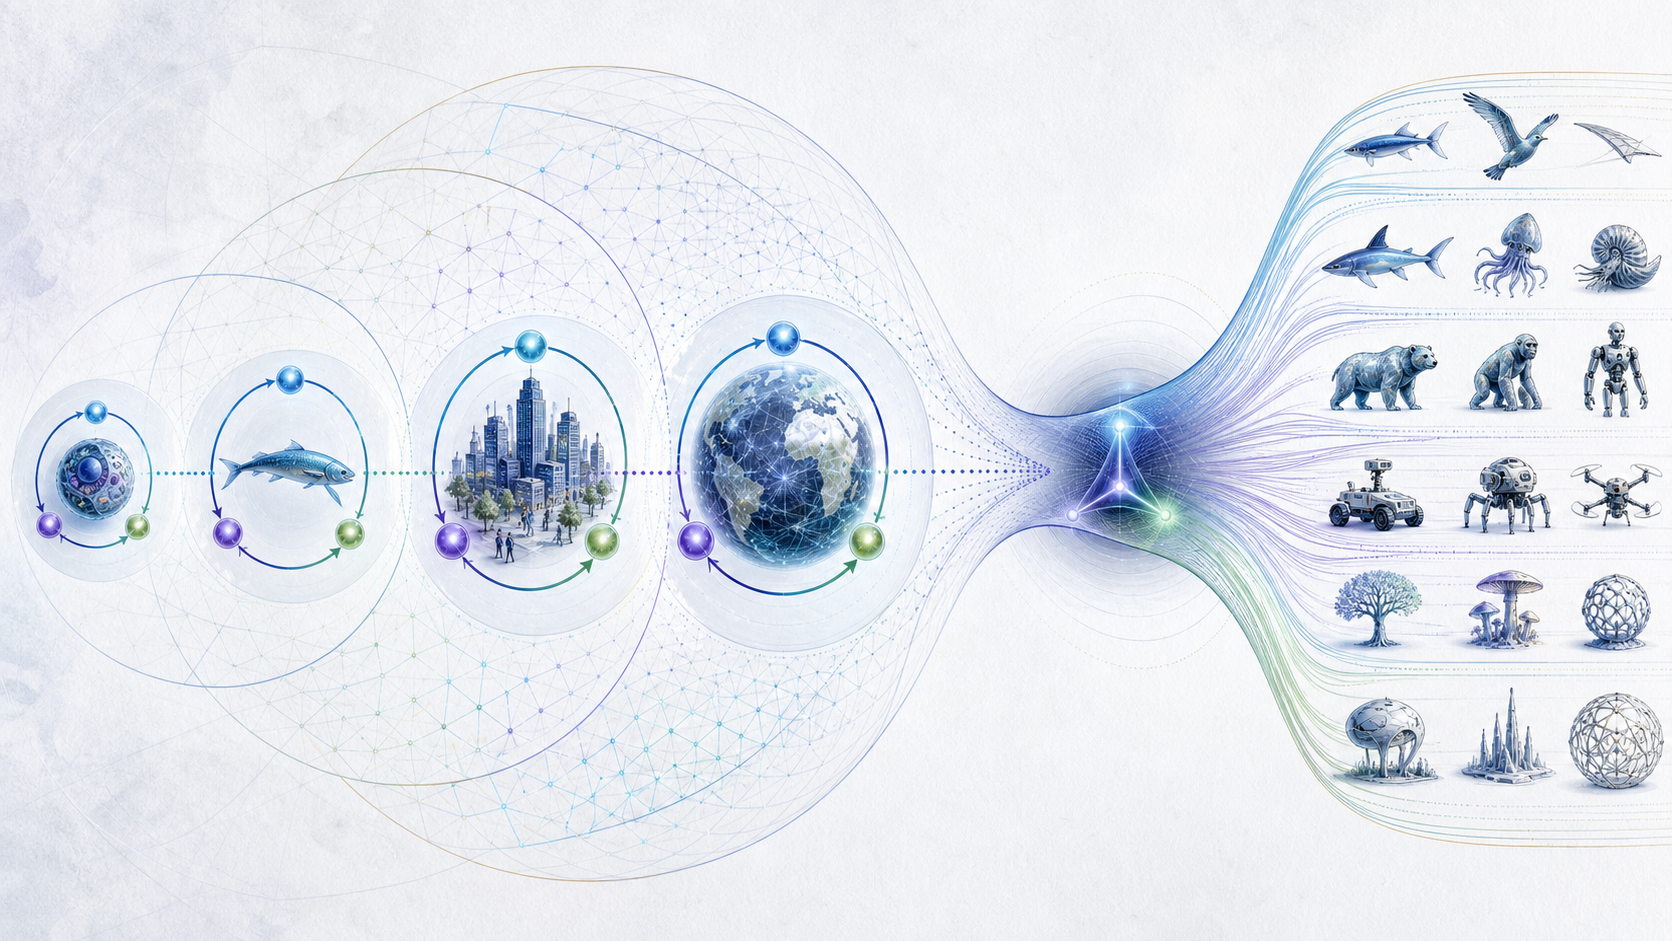
\includegraphics[width=.9\textwidth,height=.38\textheight,keepaspectratio]{images/fractal-semantic-intelligence-space.png}
\caption{跨载体语义关系与多尺度动力同构}
\end{figure}


\section{不同材料能否产生同一种智能}

当我们说两个人拥有``相同类型的智能''时，我们通常并不要求两人大脑中每一个神经元的位置、突触权重以及瞬时放电状态完全一致。事实上，即便属于同一物种的两个个体，也不可能具有完全相同的物理实现。由此立即产生一个更一般的问题：如果生物神经系统内部尚且允许巨大的实现差异，那么一个由神经元构成的生物智能与一个由数字计算构成的人工智能，是否可能在更高层意义上属于同一种智能？

这个问题要求我们首先区分\textbf{实现身份（implementation identity）}与\textbf{智能类型身份（intelligence-type identity）}。设一个智能系统记为
\[
\mathcal A=
(\mathcal X,\mathcal U,\mathcal Y,\mathcal F,\mathcal M),
\]
其中$\mathcal X$表示内部状态空间，$\mathcal U$表示输入或作用集合，$\mathcal Y$表示可观测输出，$\mathcal F$表示状态转移机制，而$\mathcal M$表示内部认知结构及其组织方式。如果另一智能系统为
\[
\mathcal B=
(\mathcal X',\mathcal U',\mathcal Y',\mathcal F',\mathcal M'),
\]
显然在现实中通常有
\[
\mathcal X\neq\mathcal X',
\qquad
\mathcal F\neq\mathcal F',
\qquad
\mathcal M\neq\mathcal M'.
\]
因此若要求两个智能系统在这些实现量上相等，跨材料智能比较从一开始就失去了意义。

本书采用的基本立场是：
\[
\boxed{
\text{Same Intelligence Type}
\not\Rightarrow
\text{Same Physical Implementation}
}
\]
更进一步，
\[
\boxed{
\text{Same Intelligence Type}
\not\Rightarrow
\text{Same Internal Representation}
}
\]
真正需要保持的，是实现之上的某些结构关系。

这与计算理论中的``多重可实现性''存在认识论上的相似性：同一个高层功能可能由不同低层机制实现。例如，对一个物体进行空间定位，可以由生物视觉系统实现，也可以由摄像头、SLAM、场景图和坐标变换算法联合实现。两者的中间状态完全不同，但在更高功能层，它们都可能建立
\[
Object
\rightarrow
Location
\rightarrow
ActionPossibility
\]
这样的结构关系。因此，若我们只关注底层材料，就会错误地把实现差异当成智能类型差异。

然而，本书并不采用一种过于宽松的功能主义，即只要``最终结果相同''就认为智能相同。因为一个简单查表程序可能在有限测试集上与具有世界模型的智能体产生相同输出，却不意味着二者拥有同类智能结构。真正的智能同类性至少涉及三层保持关系：
\begin{statementbox}
ProblemStructure
\end{statementbox}
、
\begin{statementbox}
SemanticStructure
\end{statementbox}
以及
\begin{statementbox}
DynamicalOrganization
\end{statementbox}

因此我们要寻找的不是物理同构，而是一种更高层的\textbf{认知动力学等价类}。不同物理基底可以看作对某种更抽象智能结构的具体实现。若记这种抽象智能结构为$\mathfrak I$，则多个具体系统可以分别通过实现映射
\[
\pi_A:\mathfrak I\rightarrow\mathcal A,
\qquad
\pi_B:\mathfrak I\rightarrow\mathcal B
\]
获得不同的物理形式。此时真正需要讨论的是：是否存在某种映射$\Phi$，使得$\mathcal A$与$\mathcal B$在关键认知关系上保持可交换，即
\[
\Phi\circ F_A
\approx
F_B\circ\Phi.
\]
这里的$\approx$并不意味着数值完全一致，而意味着当系统处于对应的认知状态时，它们的主要结构转移保持一致。

这一思想将在后文逐步发展为``多尺度认知动力学同构''。因此，本章的第一原则可以写为：
\begin{proposition*}
\bfseries 智能同类性的研究对象不是材料，而是跨实现仍然保持的认知组织关系。
\end{proposition*}

这一原则非常重要。它不仅允许我们比较人脑与人工智能，也允许比较完全不同的机器人身体、数字 Agent、群体智能甚至未来可能存在的异种智能。材料决定一个智能可以怎样实现，但材料本身并不足以定义这个智能属于哪一种认知结构类型。

\section{实现等价与功能等价}

如果放弃物理实现相同这一要求，我们接下来就必须回答一个更困难的问题：什么程度的``功能相同''才足以支持智能同类性的判断？这里首先需要区分至少四种不同的等价层级：输出等价、行为等价、功能等价以及认知动力学等价。

最弱的形式是\textbf{输出等价}。设两个系统在测试集合$\mathcal D$上满足
\[
\forall x\in\mathcal D,
\qquad
y_A(x)=y_B(x),
\]
那么在这个数据集上，它们具有输出等价。但这种等价非常弱，因为有限输入集合无法说明系统内部是否真正形成相同的问题结构。一个复杂模型与一个足够大的查找表可以在有限域内实现相同映射，
\[
f_A(x)=f_B(x),
\]
但它们对分布外问题、扰动、反事实以及长期学习的响应可能完全不同。

更强的是\textbf{行为等价}。这时我们不只观察一个输入产生一个输出，而观察系统在环境中的状态—行动轨迹：
\[
\Gamma_A=
(x_0,a_0,x_1,a_1,\dots),
\]
\[
\Gamma_B=
(x'_0,a'_0,x'_1,a'_1,\dots).
\]
如果存在适当的状态映射$\Phi$与行动映射$\Psi$，使得
\[
\Phi(x_t)\approx x'_t,
\qquad
\Psi(a_t)\approx a'_t
\]
并且长期闭环轨迹具有相似结构，则二者获得更强的行为等价。

这种思想与自动机理论、程序语义学中的bisimulation存在明显联系。双模拟关注两个状态转移系统之间是否存在关系$\mathcal R$，使一方发生合法状态转移时，另一方能够产生对应状态转移，并继续维持$\mathcal R$。形式上可以写为：
\[
x_A\mathcal R x_B
\]
且如果
\[
x_A\xrightarrow{a}x_A',
\]
则存在
\[
x_B\xrightarrow{b}x_B'
\]
满足
\[
x_A'\mathcal R x_B'.
\]
这种思想对智能比较极有价值，因为它把关注点从瞬时输出提升到了\textbf{状态转移结构}。

但是，智能系统比普通自动机多了一层重要结构：两个系统即使表现出类似行为，也可能是因为它们在测试环境中偶然具有相同策略，而不是因为它们形成了同类认知结构。例如，一个系统可能显式构建物体、关系、目标和风险结构，另一个系统则通过高度特化的端到端模式直接生成动作。若环境发生结构性变化，两者将表现出完全不同的泛化与学习轨迹。

因此，本书进一步定义\textbf{功能等价}。设系统包含一组高层功能：
\[
V_F^A=\{F_1^A,\dots,F_m^A\},
\qquad
V_F^B=\{F_1^B,\dots,F_n^B\}.
\]
如果存在映射
\[
\Phi_F:V_F^A\rightarrow V_F^B
\]
使得主要功能作用关系得到保持，则我们可以说二者在该功能子空间中具有等价性。例如，一个系统中的``空间定位''可能由三个神经子系统联合完成，而另一个系统中的相同功能由一个统一视觉世界模型完成，因此$\Phi_F$不必是一一映射，而可以是多对多关系。

真正进入本书理论核心的，则是第四层：
\begin{statementbox}
Cognitive Dynamical Equivalence
\end{statementbox}
也就是认知动力学等价。

它不仅要求功能闭环近似保持，还要求认知结构如何生成、激活、迁移、稳定以及在异常下重新提升具有可映射关系。如果系统$A$在技能学习过程中表现为
\[
ExplicitStructure
\rightarrow
Experience
\rightarrow
StableSkill,
\]
而系统$B$虽然底层算法完全不同，却同样表现出
\[
ExplicitStructure'
\rightarrow
Experience'
\rightarrow
StableSkill',
\]
并且存在结构映射保持这条迁移关系，那么二者才在更深层意义上可能属于同类智能。

因此智能同类性不是一个二值开关，而应看成层级关系：
\[
\resizebox{.96\linewidth}{!}{$\displaystyle
OutputEquivalence
\subset
BehavioralEquivalence
\subset
FunctionalEquivalence
\subset
CognitiveDynamicalEquivalence.
$}
\]
这里的包含关系并非严格数学集合定理，而是一种理论强度排序。

这一区分也告诉我们，传统Benchmark为什么不足以回答``两个系统是不是同类智能''。Benchmark主要测试输出和有限行为，而智能同类性真正关心的是：面对相同结构性问题时，系统是否形成类似的认知组织、是否以类似方式使用记忆、是否在异常中提升显式认知、是否能够把重复认知沉降成更稳定结构。换句话说，我们比较的不是一次计算结果，而是\textbf{形成结果的结构动力学}。

\section{面向问题的一致性}

早期讨论同类智能时，我们提出的第一条直观原则是：两个智能若要被归入同一语义类型，它们首先应该``面向相同的问题''。这里的``问题''不能被理解成一个自然语言字符串，而应被理解成一个具有目标、约束、状态与可行变换关系的结构对象。

设一个问题可以表示为
\[
\mathcal P=
(\mathcal S,
\mathcal G,
\mathcal C,
\mathcal A,
\mathcal R),
\]
其中$\mathcal S$表示状态空间，$\mathcal G$表示目标集合，$\mathcal C$表示约束，$\mathcal A$表示可行动作或变换，$\mathcal R$表示状态、目标与动作之间的关系结构。那么，两个智能系统是否面向``同一个问题''，真正需要比较的是它们内部形成的问题表示
\[
\hat{\mathcal P}_A,
\qquad
\hat{\mathcal P}_B
\]
是否都与现实问题$\mathcal P$保持足够一致的结构投影。

这可以用映射表示：
\[
\phi_A:\mathcal P\rightarrow\hat{\mathcal P}_A,
\]
\[
\phi_B:\mathcal P\rightarrow\hat{\mathcal P}_B.
\]
由于系统感知能力、身体、记忆和表征体系不同，一般不可能有
\[
\hat{\mathcal P}_A=\hat{\mathcal P}_B.
\]
真正重要的是存在某种高层关系$\Xi$，使得
\[
\Xi(\hat{\mathcal P}_A)
\approx
\hat{\mathcal P}_B
\]
并保持决定行动结果的主要问题结构。

例如，对于``绕过障碍到达目标''这一任务，人类可能内部使用视觉场、身体姿态、目标方向与运动预测进行表征；移动机器人可能使用占据栅格、SLAM位姿、轨迹代价与控制约束。两者的具体表示完全不同，但都可能抽象出：
\[
CurrentPosition,
\quad
Obstacle,
\quad
Target,
\quad
FeasiblePath
\]
之间的基本关系。因此，它们所面对的问题在更高语义层可能属于同一类。

本书进一步提出\textbf{问题语义骨架}：
\[
\Sigma_P=
(V_P,E_P,\Lambda_P),
\]
其中$V_P$是问题中的核心结构对象，$E_P$是它们之间的因果、空间、约束和目标关系，$\Lambda_P$描述哪些关系对问题求解具有决定性意义。这样，我们不再要求智能系统恢复世界的全部细节，只要求其内部问题模型保留任务充分（task-sufficient）的关系。

于是可以定义一种问题结构保持度：
\[
D_P(A,B)
=
d\left(
\Phi_A(\Sigma_P),
\Phi_B(\Sigma_P)
\right),
\]
其中$d$表示图结构或关系结构之间的距离。若
\[
D_P(A,B)<\epsilon_P,
\]
则可认为两者对该问题具有近似一致的结构理解。

但是这里必须特别注意：``面向相同问题''并不意味着``具有相同目标''。一个捕食者和逃逸者可能面对同一个空间环境，却拥有完全不同的目标函数。一个医生和病原体也可能同时作用于同一生物系统，却不能因此归为同一类智能。因此，问题一致性需要至少区分三个层次：
\[
WorldStructure,
\quad
TaskStructure,
\quad
GoalStructure.
\]
智能同类判定通常要求前两者高度可映射，而第三者是否必须一致，则取决于我们正在定义的是``认知能力类''还是``完整智能体类''。

这一点使智能分类具有明显的相对性。我们可以说两个系统都具有``路径规划智能''，即使它们长期价值和身份完全不同；但如果要判断两个完整智能体是否具有同类整体智能，仅仅共享路径规划功能显然不够。因此：
\begin{proposition*}
智能类型判定必须首先声明比较尺度。
\end{proposition*}
这个原则与前面关于智能时空尺度的讨论是一致的：任何同类性判断都必须说明究竟比较局部功能、任务级能力，还是完整生命周期智能。

面向问题的一致性因此提供了同类智能判定的第一层语义锚点。没有这一层，输出相似很容易退化为偶然相关；有了这一层，我们才能进一步讨论两个系统是否以相似方式组织行动和内部认知。

\section{行为结果的一致性}

如果问题结构相近，但两个系统产生完全不同的行动后果，我们当然很难认为它们在该能力上属于同一智能类型。因此，早期同类智能判据中的第二条是``结果相似''。然而，本书需要把``结果''从单一任务得分扩展为闭环行为结构。

设现实环境的状态为$x_t$，智能体的内部状态为$z_t$，行动为$a_t$。一般智能闭环可以表示为
\[
z_{t+1}
=
F(z_t,o_t),
\]
\[
a_t
=
\pi(z_t),
\]
\[
x_{t+1}
=
G(x_t,a_t,\eta_t),
\]
其中$o_t$是观测，$\eta_t$表示环境扰动。两个智能体$A$与$B$即使内部状态维度完全不同，我们仍然可以通过它们在相似环境中的闭环轨迹比较行为。

但只比较最终状态
\[
x_T^A\approx x_T^B
\]
仍然过于宽松。更合理的是比较一组行为不变量（behavioral invariants）。例如：
\[
GoalAchievement,
\]
\[
ConstraintViolation,
\]
\[
RecoveryBehavior,
\]
\[
ResourceCost,
\]
\[
Robustness,
\]
\[
AdaptationRate.
\]
我们可以把这些指标组成行为特征向量
\[
\mathbf b_A
=
(b_1^A,\dots,b_k^A),
\]
并定义行为距离
\[
D_B(A,B)
=
\|\mathbf b_A-\mathbf b_B\|_W,
\]
其中$W$表示各项特征的重要度。

但智能行为还有一个非常关键的维度：\textbf{面对扰动以后如何恢复}。如果两个系统在正常任务上表现一致，但一个系统在遭遇异常后能够重新识别问题、提升显式推理并找到替代方案，而另一个系统立即崩溃，那么它们在认知结构上并不应被视为完全同类。

因此行为比较应覆盖一组扰动族：
\[
\Delta=
\{\delta_1,\delta_2,\dots,\delta_n\}.
\]
对于每个扰动$\delta_i$，观察：
\[
\Gamma_A^{(\delta_i)},
\qquad
\Gamma_B^{(\delta_i)}.
\]
如果二者不仅正常轨迹相似，而且在扰动、恢复、重新规划和再学习方面具有对应关系，那么行为等价的可信度大幅增强。

由此可以进一步定义行为等价概率：
\[
P_{\mathrm{beh}}(A\sim B)
=
\mathbb E_{\mathcal E,\Delta}
\left[
K(
\Gamma_A,
\Gamma_B
)
\right],
\]
其中$\mathcal E$是环境分布，$K$是轨迹相似核。这个形式强调：智能同类性不应该基于一次测试，而应基于一个环境族和扰动族上的系统行为。

同时，本书需要警惕另一个错误：把行为结果一致性直接等同于认知同一性。一个系统可能通过世界模型、预测和规划完成任务，另一个可能通过大量记忆样例匹配完成相同任务。只要任务分布足够窄，它们可能表现相同。但当问题进入新组合、反事实或长时适应时，两者的内部差异会显现。

因此我们可以写：
\[
\boxed{
BehavioralSimilarity
\text{ is necessary evidence, but not sufficient proof of cognitive equivalence.}
}
\]
在同类智能判定中，行为结果的作用是提供现实约束，因为智能理论最终必须接受现实反馈检验；但它必须与下一节讨论的``语义结构一致性''联合使用。

这一点与本书始终坚持的原则一致：
\begin{statementbox}
RealityIsUltimateConstraint.
\end{statementbox}
认知结构无论多么漂亮，如果不能在现实闭环中产生相应行为，其所谓``同类性''就失去了功能基础；反过来，行为相似如果没有稳定内部结构支持，也不能自动提升为强认知等价。

\section{语义关系的一致性}

面向问题的一致性告诉我们两个系统是否在处理大致相同的问题，行为一致性告诉我们它们是否产生大致相同的现实结果，但这两层仍然无法回答一个更加核心的问题：它们是否以相似的\textbf{认知结构关系}理解和组织这个问题？

这正是本书提出CSO之后，同类智能理论发生的重要升级。

设智能体$A$内部当前激活的认知结构图为
\[
\mathcal G_C^A
=
(V_C^A,E_C^A),
\]
其中每个节点是一个Agent-CSO，而边可以具有不同语义类型：
\[
E_C
=
E^{causal}
\cup
E^{spatial}
\cup
E^{temporal}
\cup
E^{goal}
\cup
E^{constraint}
\cup
E^{self}
\cup
E^{value}.
\]
智能体$B$具有另一张图
\[
\mathcal G_C^B.
\]
我们不要求：
\[
V_C^A=V_C^B
\]
或
\[
E_C^A=E_C^B,
\]
因为两个实现内部使用的表示粒度可能完全不同。真正需要的是存在一个语义映射
\[
\Phi_C:
\mathcal G_C^A
\rightarrow
\mathcal G_C^B
\]
使关键结构关系得到保持。

例如，在$A$中存在因果关系：
\[
C_1
\xrightarrow{cause}
C_2,
\]
则映射之后应满足：
\[
\Phi_C(C_1)
\xrightarrow{cause'}
\Phi_C(C_2),
\]
其中$cause'$不要求采用相同数据结构，但在目标问题中承担相同因果作用。

类似地，如果
\[
C_{obstacle}
\xrightarrow{constraint}
C_{path},
\]
那么另一个系统中也必须存在某种对应结构，使障碍对可行路径产生约束。若第二个系统完全不存在这一关系，而只是通过统计相关输出动作，则两者的语义结构等价程度就应降低。

因此可以定义语义关系保持函数：
\[
\mathcal R_S
(\Phi_C,e)
\in[0,1],
\]
表示边$e$经过映射之后的语义保持程度。整体语义保持度可以写成
\[
S_C(A,B)
=
\sum_{e\in E_C^A}
w_e
\mathcal R_S
(\Phi_C,e),
\]
其中$w_e$表示该关系对当前智能能力的重要度。

这里引出了一个很重要的思想：并不是所有内部结构都同等重要。两个智能体无需在无关细节上保持同构，只需保持\textbf{因果功能上决定该智能能力的关系骨架}。我们可以将这一骨架表示为
\[
\mathcal G_C^\star
\subseteq
\mathcal G_C,
\]
称为\textbf{核心语义子图}。

所谓同类智能，真正要求的是存在
\[
\Phi_C:
\mathcal G_C^{A\star}
\rightarrow
\mathcal G_C^{B\star}
\]
保持关键语义关系，而不是整个内部状态空间逐点对应。

这一理论与知识图谱同构、图匹配、frame semantics以及关系表示理论存在外部关联，但本书进一步要求这些语义图必须进入行动闭环。一个纯数据库也可以保存``物体—位置—关系''，但如果这些关系不能影响预测、决策和学习，就不能仅凭结构相似判断它具有同类智能。

因此我们还必须要求：
\[
SemanticRelation
\rightarrow
FunctionalConsequence.
\]
即一个被认为重要的Agent-CSO关系必须在系统动力学中具有可识别的因果作用。例如改变``目标''节点应改变行动倾向，改变``障碍''节点应改变路径选择，改变``自我能力''节点应改变可行动作集合。否则这些语义只是附加标签，而不是认知结构。

从这一点出发，本书可以提出一个非常强的同类智能原则：
\begin{proposition*}
\bfseries
真正的语义等价不是两个系统拥有相似标签，而是相应语义结构在各自系统中具有相似的因果功能。
\end{proposition*}
也就是说：
\[
SemanticEquivalence
=
RelationalSimilarity
+
CausalRoleSimilarity.
\]

这一原则使我们的语义类规约超出了传统ontology matching。它不只比较``这个概念叫什么''，而比较``这个概念在整个智能闭环中做什么''。这为下一节正式定义Semantic Class奠定基础。

\section{Semantic Class：语义类规约}

有了问题结构、行为轨迹和认知语义关系三个层面，我们可以正式定义本书所谓的``语义类''。语义类不是一组具有相同内部表示的系统，而是一组在指定认知尺度上保持关键语义—功能关系的智能实现。

设一个智能能力类型$\mathfrak C$由如下规范描述：
\[
\mathfrak C
=
(
\Sigma_P,
\Sigma_C,
\Sigma_F,
\Sigma_D
),
\]
其中：

\[
\Sigma_P
\]
表示问题结构规约；

\[
\Sigma_C
\]
表示核心CSO语义规约；

\[
\Sigma_F
\]
表示功能闭环规约；

\[
\Sigma_D
\]
表示主要动力学约束。

则对于具体智能体$A$，若存在一组映射
\[
\Phi_P^A,
\quad
\Phi_C^A,
\quad
\Phi_F^A
\]
使其具体实现满足这些规约到足够精度，我们就可以写：
\[
A\models_{\epsilon}\mathfrak C.
\]
这里$\epsilon$表示允许的实现差异。

由此定义语义类：
\[
\boxed{
[\mathfrak C]_{\epsilon}
=
\{
A\mid A\models_{\epsilon}\mathfrak C
\}.
}
\]

这意味着``智能类型''不再是一个模糊标签，而可以被理解成一组约束条件所定义的实现等价类。

例如，一个``目标导向空间导航智能''的Semantic Class可能要求至少存在：

当前位置CSO；

目标CSO；

障碍/约束CSO；

可行动作结构；

空间预测；

路径评价；

行动后反馈；

残差驱动更新。

具体系统是否使用海马体、Transformer、occupancy grid、latent world model或者其他表示，并不进入该Semantic Class最核心的规定，只要关键关系和闭环被满足。

因此：
\[
\boxed{
SemanticClass
\neq
ImplementationClass.
}
\]

这也意味着一个智能体可以同时属于多个语义类。例如系统$A$可以满足导航类$\mathfrak C_1$、社会协调类$\mathfrak C_2$以及工具使用类$\mathfrak C_3$：
\[
A
\in
[\mathfrak C_1]
\cap
[\mathfrak C_2]
\cap
[\mathfrak C_3].
\]
完整智能体可以被理解成多个Semantic Class的组合、耦合和跨尺度协调。

这与我们前一章提出的``智能空间与智能的基''产生直接联系。如果存在一组基础语义功能类
\[
\{\mathfrak C_1,\dots,\mathfrak C_n\},
\]
那么一个具体智能系统可以表示为：
\[
\mathfrak I_A
=
\bigoplus_i
\alpha_i\mathfrak C_i
+
\mathcal R_A,
\]
其中$\mathcal R_A$表示这些智能类之间的组织关系。这里的$\oplus$不是普通线性代数加法，而表示结构组合。

从这个角度，同类智能判定不再只有：
\[
A\sim B
\]
这样的整体问题，而可以分解为：
\[
A\sim_{\mathfrak C_i}B,
\]
即``A与B在智能类$\mathfrak C_i$上是否等价''。

这种局部化非常重要。一个人类与自动驾驶系统显然不是整体同类智能，但它们在某些视觉预测、目标追踪或局部空间推理类上可能存在部分语义等价。类似地，一个大型语言模型与人类的完整生命体结构差别巨大，但在某些语言推理Semantic Class中仍可能存在强对应关系。

这也使``人工智能是否和人一样智能''这种宽泛问题失去必要性。更严格的问题应改写成：
\begin{statementbox}
两个系统在哪些Semantic Classes中具有多高程度的结构等价？
\end{statementbox}

为了量化这种关系，可以定义：
\[
S_{\mathfrak C}(A,B)
=
\alpha S_P
+
\beta S_C
+
\gamma S_F
+
\delta S_D,
\]
满足
\[
\alpha+\beta+\gamma+\delta=1.
\]
其中分别衡量问题结构、语义结构、功能闭环和动力学结构的相似程度。

于是智能类不再是绝对分类，而可以出现连续程度：
\[
0
\le
S_{\mathfrak C}(A,B)
\le
1.
\]
这比单纯使用``像人''或者``不像人''的语言更加适合未来异构智能研究。

但Semantic Class仍然不是本章的终点。因为两个系统即使具有类似语义和功能结构，如果它们在时间尺度组织、学习迁移和上下层反馈方面完全不同，其长期智能性质仍可能不同。因此，我们还需要引入最后一个更强条件：多尺度认知动力学同构。

\section{多尺度认知动力学同构}

前面的同类性条件主要关注``什么结构被保持''，但智能真正特殊之处在于这些结构不是静止存在，而是在时间中持续生成、激活、迁移、稳定和重组。因此，最强形式的智能同类判定必须加入时间尺度。

设智能体$A$具有认知图
\[
\mathcal G_C^A(t)
\]
和功能图
\[
\mathcal G_F^A(t),
\]
以及承载映射
\[
\mu_t^A:
\mathcal G_C^A
\rightarrow
\mathcal G_F^A.
\]
智能体$B$对应为
\[
\mathcal G_C^B(t'),
\qquad
\mathcal G_F^B(t'),
\qquad
\mu_{t'}^B.
\]

若存在语义映射
\[
\Phi_C:
\mathcal G_C^A
\rightarrow
\mathcal G_C^B
\]
和功能映射
\[
\Phi_F:
\mathcal G_F^A
\rightarrow
\mathcal G_F^B,
\]
并存在时间重参数化
\[
t'=g(t),
\qquad
\frac{dg}{dt}>0,
\]
使得以下关系近似成立：
\[
\Phi_F\circ\mu_t^A
\approx
\mu_{g(t)}^B\circ\Phi_C,
\]
那么两个系统在某一时刻的``什么认知结构由什么功能承载''这一关系得到保持。

但我们还需要动力学可交换条件。若系统演化算子分别为
\[
\mathcal D_A,
\qquad
\mathcal D_B,
\]
则要求：
\[
\boxed{
\Phi
\circ
\mathcal D_A
\approx
\mathcal D_B
\circ
\Phi
}
\]
其中
\[
\Phi=
(\Phi_C,\Phi_F,g).
\]

这意味着：先让系统$A$演化再做映射，与先映射到系统$B$再让$B$按照自己的动力学演化，最终应获得近似对应的结构。

这正是我们所称的：
\begin{statementbox}
MultiscaleCognitiveDynamicalIsomorphism
\end{statementbox}
即\textbf{多尺度认知动力学同构}。

特别重要的是，这种同构允许两个系统速度完全不同。设系统$A$中的某类过程频率为$\omega_A$，系统$B$为$\omega_B$，只需要存在单调尺度映射：
\[
\omega_B
=
g_\omega(\omega_A).
\]
例如，一个生物神经系统完成某种技能自动化可能需要数天，而一个数字Agent可能在数分钟内完成对应结构迁移。若二者都表现出：
\[
ExplicitCSO
\rightarrow
RepeatedExperience
\rightarrow
StableProceduralCSO,
\]
那么其绝对时间不同并不妨碍动力学结构同类。

因此：
\[
\boxed{
SameTimescalePattern
\neq
SameClockSpeed.
}
\]
更合理的判据是相对尺度次序得到保持。例如：
\[
\tau_{fast}
\ll
\tau_{working}
\ll
\tau_{memory}
\ll
\tau_{self}
\]
在另一个系统中映射为：
\[
\tau'_{fast}
\ll
\tau'_{working}
\ll
\tau'_{memory}
\ll
\tau'_{self}.
\]
只要相对层级与跨层作用方式类似，绝对秒数可以完全不同。

我们还可以进一步要求关键迁移模式保持。例如系统$A$具有：
\[
StableStructure
\rightarrow
Lower/FasterCarrier
\]
和
\[
PersistentResidual
\rightarrow
Higher/SlowerProcessing.
\]
若$B$也存在对应关系，则二者不仅在静态功能上相似，而且在``成熟能力如何下沉、异常如何上浮''这一学习动力学上相似。

因此最强智能同类判据实际上包括四个保持条件：
\begin{statementbox}
SemanticPreservation
\end{statementbox}
、
\begin{statementbox}
FunctionalLoopPreservation
\end{statementbox}
、
\begin{statementbox}
TimescaleOrderPreservation
\end{statementbox}
以及
\begin{statementbox}
MigrationLawPreservation.
\end{statementbox}

可以将总同构误差写为：
\[
\mathcal E_{\mathrm{iso}}
=
\lambda_C E_C
+
\lambda_F E_F
+
\lambda_\tau E_\tau
+
\lambda_M E_M.
\]
若
\[
\mathcal E_{\mathrm{iso}}
<
\epsilon_{\mathrm{class}},
\]
则我们可以在指定语义类和尺度下，将两个系统视为近似同类智能。

这里必须强调``近似''。真实复杂智能系统几乎不可能实现严格数学同构，因此我们讨论的是结构保持意义下的弱同构、近似同构或同类动力学，而不是逐点双射。

外部理论中，bisimulation提供状态转移等价的数学直觉；system identification帮助我们从输入输出反推动力结构；图同态帮助定义结构保持；computational functionalism提供实现独立性的哲学背景。但本书在这些理论之上额外要求了\textbf{CSO语义关系、功能拓扑与多尺度迁移规律同时保持}，因此这一理论属于本书智能动力学框架自身的扩展。

\section{为什么神经系统与Transformer可以进行跨实现比较}

完成上述理论以后，我们终于可以重新回答一个现实中非常常见、但通常被问得过于粗糙的问题：人脑中的神经系统和Transformer是否具有可比较性？

严格而言，``人脑等不等于Transformer''不是一个良定义问题。人脑是具有身体、内稳态、长期记忆、自我、社会历史和生命周期的完整生物系统，而一个普通Transformer通常只是一个特定计算模型。因此如果比较对象的尺度不同，
\[
SystemScale_A
\neq
SystemScale_B,
\]
整体等价问题从一开始就失效。

正确做法是首先选择Semantic Class。

例如我们可以只比较：
\[
\mathfrak C_{\mathrm{sequence}}
\]
序列关系建模；

或者：
\[
\mathfrak C_{\mathrm{context}}
\]
上下文依赖预测；

或者：
\[
\mathfrak C_{\mathrm{relational}}
\]
关系结构形成；

再或者：
\[
\mathfrak C_{\mathrm{planning}}
\]
目标约束下的状态转移推理。

在这些局部语义类上，完全可以研究两个系统是否形成类似的功能动力学。

例如对于预测问题，可以抽象出：
\[
Context
\rightarrow
InternalState
\rightarrow
Prediction
\rightarrow
Error
\rightarrow
Update.
\]
生物系统可能通过神经动力学、突触可塑性和多脑区闭环完成；人工系统可能通过attention、latent state、external memory以及梯度或上下文更新完成。实现方式完全不同，但若其关键语义—功能关系具有对应，就具有可比较基础。

同样，对于长期记忆形成，我们真正比较的也不应该是``海马体对应Transformer哪一层''。这种一一器官映射通常是错误方向。更合理的问题是：
\begin{statementbox}
两个系统是否都存在从快速当前状态到较慢经验结构，再到长期生成结构的迁移？
\end{statementbox}
如果存在，则可以比较：
\[
FastState
\rightarrow
Trajectory
\rightarrow
SlowStructure
\]
这一动力学模式，而无需断言：
\[
Hippocampus
=
VectorDatabase.
\]

这一方法可以有效避免人工智能研究中常见的``生物器官机械类比''。本书并不认为某个AgentOS模块就是大脑某个区域，而是认为二者可能在某些尺度上实现同一类功能闭环。

例如SPC与某些自我状态估计网络可能存在功能类似性，但：
\[
SPC\neq DMN.
\]
AHC与生物内稳态/神经调制系统可能有结构启发关系，但：
\[
AHC\neq LimbicSystem.
\]
BPCC可以借鉴小脑式快速预测控制思想，但：
\[
BPCC\neq BiologicalCerebellum.
\]
同理，Transformer与皮层也不应进行简单等号映射。

我们真正需要寻找的是：
\begin{statementbox}
FunctionalCorrespondence
\end{statementbox}
和
\begin{statementbox}
DynamicalCorrespondence.
\end{statementbox}

从数学上，可以分别建立人类系统$H$与人工系统$M$的核心语义图：
\[
\mathcal G_C^H,
\qquad
\mathcal G_C^M,
\]
功能图：
\[
\mathcal G_F^H,
\qquad
\mathcal G_F^M,
\]
以及时间尺度谱：
\[
\mathcal T_H
=
\{\tau_1^H,\dots,\tau_m^H\},
\]
\[
\mathcal T_M
=
\{\tau_1^M,\dots,\tau_n^M\}.
\]
然后寻找：
\[
\Phi_C,
\quad
\Phi_F,
\quad
g_\tau
\]
是否能够保持一个指定Semantic Class中的主要关系。

因此，对跨实现智能研究而言，一个比``Transformer像不像大脑''更加科学的问题是：
\begin{statementbox}
在给定认知语义类中，人脑与人工系统是否存在可识别的多尺度动力学映射？
\end{statementbox}

这一问题是可研究、可比较、甚至可以逐渐实验化的。

进一步说，本章提出的同类智能理论还为未来异构智能社会提供了一个基础。如果我们有生物人类、数字Agent、机器人Agent以及可能完全不同材料构成的智能系统，仅凭材料分类将无法回答它们是否真正能够共享某些认知协议。语义类规约则允许我们定义：
\[
\mathfrak C_{\mathrm{communication}},
\qquad
\mathfrak C_{\mathrm{causal}},
\qquad
\mathfrak C_{\mathrm{social}},
\qquad
\mathfrak C_{\mathrm{self}},
\]
并分别检验不同系统之间是否存在结构映射。

因此，本章最终得到的不是``所有智能都是一样的''，而恰恰是一个更加严格的判断框架：
\begin{proposition*}
\bfseries
智能既不能因为实现不同而被轻易判为异类，也不能因为行为相似而被轻易判为同类。
\end{proposition*}

真正的同类性需要我们在指定尺度和指定Semantic Class中同时考察：
\[
\boxed{
Problem
+
Behavior
+
SemanticStructure
+
FunctionalTopology
+
TimescaleDynamics.
}
\]

由此可以将本章的最终判定关系写成：
\[
\boxed{
A
\sim_{\mathfrak C,\epsilon}
B
}
\]
当且仅当在语义类$\mathfrak C$中存在一组近似结构映射
\[
\Phi
=
(
\Phi_P,
\Phi_C,
\Phi_F,
g_\tau
)
\]
使问题结构、关键Agent-CSO关系、功能闭环以及多尺度演化规律均在容许误差$\epsilon$内得到保持。

这就是本书所谓的\textbf{同类智能判定原理}。

它使我们能够跨越神经元、Transformer、机器人、数字Agent以及未来未知物理实现，讨论一个比``材料是否相同''更加基础的问题：\textbf{这些系统是否在以同一种认知动力学形式面对世界。}

而这也自然引向下一章的问题：如果我们已经能够把智能中的基本语义结构抽离具体实现，那么究竟什么才是这些智能真正操作、迁移和稳定的基本结构对象？这一问题将在后续关于CSO本体及其具体承载形式的讨论中得到进一步形式化。
